\chapter{Functors}

\textbf{FUNCTORS PRESERVE ISOMORPHISMS? CHECK,WRITE ABOUT}
Another central definition in Category Theory is that of Functors.
While morphisms relate objects inside a category, a Functor
establishes a relation between categories, thus, it's one level
higher in terms of abstraction.


\section{What is a Functor?}

Let's formally define a Functor.

\begin{definition}[Functor]
	Let $\mathcal C$ and $\mathcal D$ be two categories. A functor $F: \mathcal C \to \mathcal D$ is
	a pair of mappings with the following properties:
	\begin{enumerate}[(i)]
		\item a mapping between objects
		      \begin{displaymath}
			      F:Ob_\mathcal C \to Ob_\mathcal D,
		      \end{displaymath}
		      where for each $A \in Ob_\mathcal C$, $F(A) \in Ob_\mathcal D$.
		\item a mapping between morphisms
		      \begin{displaymath}
			      F:Mor_\mathcal C \to Mor_\mathcal D,
		      \end{displaymath}
		      where there are two possibilities:
		      \begin{enumerate}
			      \item \textbf{Covariant Functor}, in which
			            \begin{displaymath}
				            F:Mor_\mathcal C(A,B) \to Mor_\mathcal D (F(A),F(B)),
			            \end{displaymath}
			            hence for a morphism $f:A \to B$, then $F(f):F(A) \to F(B)$.
			      \item \textbf{Contravariant Functor}, in which
			            \begin{displaymath}
				            F:Mor_\mathcal C(A,B) \to Mor_\mathcal D (F(B),F(A)),
			            \end{displaymath}
			            hence for a morphism $f:A \to B$, then $F(f):F(B) \to F(A)$.
		      \end{enumerate}
		\item Identities morphisms are preserved, i.e. for $A \in Ob_\mathcal C$
		      \begin{displaymath}
			      F(id_A) =  id_{F(A)}.
		      \end{displaymath}
		\item Compositions are preserved, i.e. for $f \in Mor_\mathcal C(A,B)$
		      and $ g \in Mor_\mathcal C(B,C)$,
		      \begin{enumerate}
			      \item For a \textbf{Covariant Functor},
			            \begin{displaymath}
				            F(g \circ f) = F(g) \circ F(f).
			            \end{displaymath}
			      \item For a \textbf{Contravariant Functor},
			            \begin{displaymath}
				            F(g \circ f) = F(f) \circ F(g).
			            \end{displaymath}
		      \end{enumerate}
	\end{enumerate}
	It's common for authors to refer to covariant functors only as functors, i.e.
	whenever someone say that $F$ is a functor, it might be implied that it's a covariant functor.
	We'll also use this convention whenever it's not ambiguous, and we'll always.
	Also, we'll sometimes use $FA$ to mean $F(A)$.
	\label{def:functor}
\end{definition}

\begin{lemma}[Contravariant Functor]
	The definition \ref{def:functor} of covariant functor is equivalent to
	saying that	$F$ is a (covariant) functor from $\mathcal C^{\text{op}}$ to $\mathcal D$.
	\label{lemma:contravariant}
\end{lemma}
\begin{proof}
	To prove this, we need to show that for any contravariant functor $F:\mathcal C \to \mathcal D$
	defined as in \ref{def:functor}, there is an equivalent functor $F':\mathcal C^{op}\to \mathcal D$,
	and vice-versa.

	For every $A \in Ob_\mathcal C$, make $F(A) = F'(A)$. This is fine, since
	$A \in Ob_\mathcal C \iff A \in Ob_{\mathcal C^{op}}$.
	Next, for $f \in Mor_\mathcal C (A,B)$, make
	$F f = F' f^{op}$, where $f^{op}$ is the reversed morphism $f$. Again, this is well defined since
	$f \in Mor_\mathcal C(A,B) \iff f^{op} \in Mor_{\mathcal C^{op}}(B,A)$.

	Lastly, note that
	\begin{displaymath}
		(g \circ f)^{op} = f^{op} \circ g^{op},
	\end{displaymath}
	hence:
	\begin{displaymath}
		F(g \circ f) = F'(f^{op}\circ g^{op})  \iff F f \circ F g  = F' f^{op} \circ F' g^{op}.
	\end{displaymath}
	Thus, we showed that $F$ is a contravariant functor according to \ref{def:functor}
	if and only if $F'$ is a covariant functor from $\mathcal C^{\text{op}}$ to $\mathcal D$, where
	$F$ and $F'$ are the same up to an isomorphism from $\mathcal C$ to $\mathcal C^{op}$.
\end{proof}

Again, the use of diagrams may help understand what is going on. The figure below
illustrates the identity and composition preservation of Functors.

\begin{figure}[H]
	\begin{center}
		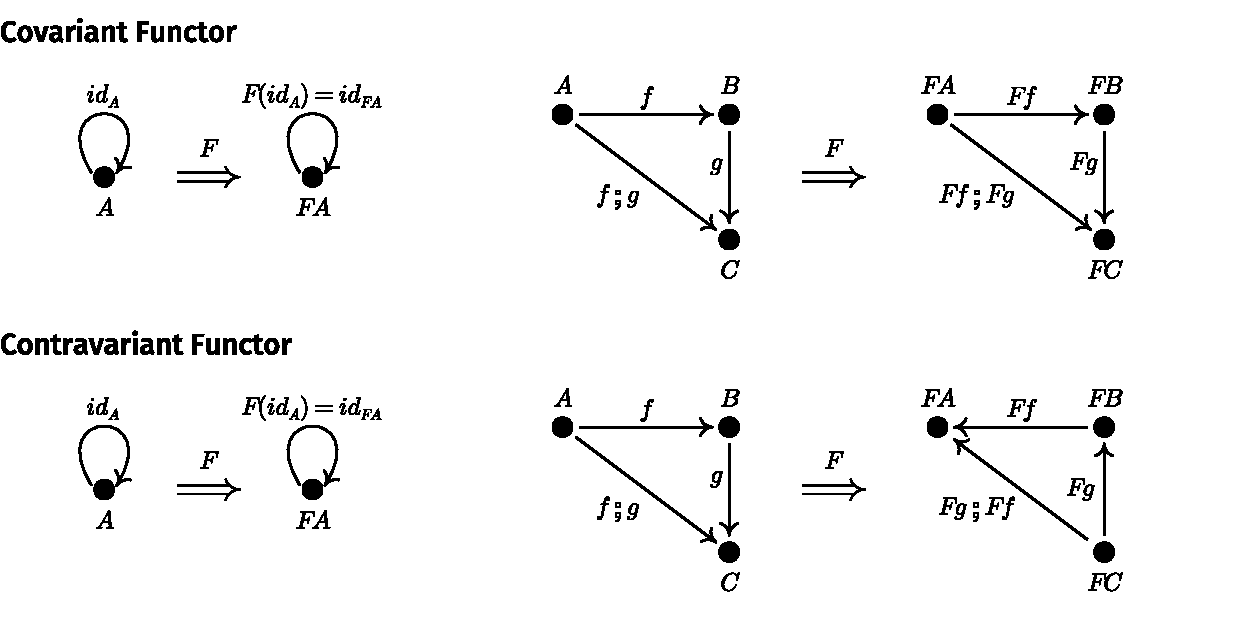
\includegraphics[width=1.1\textwidth]{./notebooks/Functor.pdf}
	\end{center}
	\caption{Diagrams showcasing the properties of Functors.}
	\label{fig:Functor}
\end{figure}

\begin{example}[Power set functors]
	An example of (covariant) functor is the functor
	$P : \mathbf{Set} \to \mathbf{Set}$, which sends a set $A$
	to it's power set $2^A$, and sends functions (the morphisms in the case
	of the category of sets) to their image set, i.e. for $f:A \to B$,
	we have $Ff:2^A \to 2^B$ such that for $X \in 2^A$ then $Ff(X) = \{f(x) : x \in X\}$.

	An example of \textbf{contravariant} functor is the inverse image functor
	$F : \mathbf{Set} \to \mathbf{Set}$, which sends a set $A$ to it's
	power set $2^A$, but sends $f$ to the inverse image, i.e.
	$Ff(Y) = \{x \in A : f(x) \in Y\}$.
	Note that the inverse image satisfy the contravariant property
	\begin{displaymath}
		F(f \circ g) = (f \circ g) ^{-1} = g^{-1} \circ f^{-1}.
	\end{displaymath}
\end{example}

\section{Category of Small Categories}

One might realize that functors are acting on categories in a very similar way as morphisms
do to objects. Indeed, we can define a functor composition.

\begin{definition}[Functor composition]
	For two functors $F:\mathcal C \Rightarrow \mathcal D$
	and $G:\mathcal D \Rightarrow \mathcal E$, then $G \circ F$ is
	a functor from $\mathcal C$ to $\mathcal E$ where
	\begin{enumerate}[(i)]
		\item For any $A \in Ob_\mathcal C$, $G\circ F (A) = G(F(A))$,
		\item For any $f \in Mor_\mathcal C$, $G\circ F (f) = G(F(f))$.
	\end{enumerate}
\end{definition}
We can also define an identity functor $I:\mathcal C \Rightarrow \mathcal C$,
where $F(A) = A$ and $F(f) = f$.

Therefore, we might wonder whether there exists a category of all categories
where objects are categories and morphisms are functors.
The answer is ``no''. Similar to the set of all sets, it can be proven
that this category does not exists. Yet, the category of all \textit{small categories}
does.

Remember, a small category is one where both morphisms and objects are sets.
With this, let's prove our first theorem.
\begin{theorem}[Category of Small Categories]
	Let $Ob_{\textbf{SmCat}}$ be small categories and $Mor_{\textbf{SmCat}}$ be functors.
	This constitutes a category.
\end{theorem}
\begin{proof}
	To prove this, we'll use the fact that in Gödel-Bernays class set theory, the
	axiom \ref{axiom:gb} implies what is called a \textit{comprehension scheme}.
	\begin{proposition}[Comprehension Scheme from \citet{borceux1994handbook}]
		If $\phi(x_1,...,x_n)$ is a formula that the quantification occurs on set variables, then
		there exists a class $A$ such that
		\begin{displaymath}
			(x_1,...,x_n) \in A \iff \phi(x_1,...,x_n).
		\end{displaymath}
	\end{proposition}
	Note that
	\begin{displaymath}
		\mathcal C := \langle Ob_\mathcal C, Mor_\mathcal C \rangle \in \textbf{SmCat} \iff
		\mathcal C \text{ ``is a category''}.
	\end{displaymath}
	Since every $\mathcal C$ is small, then the formula to check whether $\mathcal C$ is a category
	iterates over set variables, i.e. $Ob_\mathcal C$ and $Mor_\mathcal C$.
	Thus, the Comprehension Scheme proposition guarantees that $\textbf{SmCat}$ exists.
\end{proof}

\section{Types of Functors}

Before we go on to provide examples of functors, let's present
a way to classify different functors.

\begin{definition}[Faithful, Full, Fully Faithful and Embedding]
	Here we follow \citet{roman2017introduction}.
	Let $F$ be a functor between categories $\mathcal C$ and $\mathcal D$.
	\begin{enumerate}[1.]
		\item $F$ is \textbf{faithful} if for every $A,B \in Ob_\mathcal C$,
		      $F:Mor_\mathcal C(A,B)\to Mor_\mathcal C(FA,FB)$ is injective.
		\item $F$ is \textbf{full} if for every $A,B \in Ob_\mathcal C$,
		      $F:Mor_\mathcal C(A,B)\to Mor_\mathcal C(FA,FB)$ is surjective.
		\item $F$ is \textbf{fully faithful} if for every $A,B \in Ob_\mathcal C$,
		      $F:Mor_\mathcal C(A,B)\to Mor_\mathcal C(FA,FB)$ is bijective.
		\item $F$ is an \textbf{embedding} of $\mathcal C$ in $\mathcal D$ if $F$ is fully faithful
		      and $F:Ob_\mathcal C \to Ob_\mathcal D$ is injective.
	\end{enumerate}

\end{definition}

\section{Subcategories}

\begin{definition}[Subcategory]
	Let $\mathcal D$ be a category. We say that $\mathcal C$
	is a subcategory of $\mathcal D$ if $Ob_\mathcal C \subset Ob_\mathcal D$ and
	$Mor_\mathcal C \subset Mor_\mathcal D$, such that $\mathcal C$ is a category.

	If for every $A, B \in Ob_\mathcal C$, we have that $Mor_\mathcal D (A,B) = Mor_\mathcal C(A,B)$,
	then $\mathcal C$ is a \textit{full subcategory}.
\end{definition}

From the definition of a functor, one might wonder whether for any
functor $F:\mathcal C \Rightarrow \mathcal D$,
the image $F(\mathcal C)$ is a subcategory of $\mathcal D$, i.e.
if $\langle Ob_{F(\mathcal C)}, Mor_{F(\mathcal C)} \rangle$ is a category where
\begin{displaymath}
	Ob_{F(\mathcal C)}:= \{F(A) : A \in Ob_\mathcal C\}, \quad
	Mor_{F(\mathcal C)}:= \{F(f) : f \in Mor_\mathcal C\}.
\end{displaymath}
The answer is no.

\section{Relevant Examples of Functors}

Now that we know what a functor is, let's showcase some relevant examples
that might be useful to someone applying Category Theory to another field.

\begin{example}[Power Set Functor]
	The power set functor $\mathcal P : \mathbf{Set} \to \mathbf{Set}$ takes a
	set to it's power set and a function $f:A\to B$ to the image function
	$Im f : \mathcal P(A) \to \mathcal P(B)$, i.e. for a subset $S \subset A$
	in the domain, returns $f(S) := \{ f(x) \ : x \in S\}$.

	Another even more relevant example is the \textit{contravariante} power set
	functor $F : \mathbf{Set} \to \mathbf{Set}$ that takes $A$ to $\mathcal P(A)$
	and $f$ to the inverse image $f^{-1}$.
\end{example}

\begin{example}[Identity Functor]
	This does what one might expect from the name. The identity
	functor is $1_\mathcal C : \mathcal C \to \mathcal C$, such that
	$1_\mathcal C (A) = A \in Ob_\mathcal C$ and
	$1_\mathcal C (f) = f \in Mor_\mathcal C$.
\end{example}

\begin{example}[Inclusion Functor]
	For a subcategory $\mathcal S$ of $\mathcal C$, the inclusion
	functor is $I_\mathcal C : \mathcal S \to \mathcal C$, such that
	$I_\mathcal C (A \in Ob_\mathcal S) = A \in Ob_\mathcal C$ and
	$I_\mathcal C (f \in Mor_\mathcal S) = f \in Mor_\mathcal C$.
\end{example}

\section{Formalizing Diagrams}

We've drawn many diagrams representing either categories or portions of categories. Up
until now, this has been done in a informal way. Yet, it's possible to define such diagrams rigorously.
One of the reasons that formal diagrams are useful is that they allow us to talk about portions
of some category $\mathcal C$ in a rigorous manner.

\begin{definition}[Diagram]
	A $\mathcal I$-diagram (or just diagram) $D$ of a category $\mathcal C$ is a functor
	$D: \mathcal I \to \mathcal C$, where $\mathcal I$ is called the index category.
\end{definition}

The definition above is pretty much a ``placeholder'', i.e. any functor can be seen as
a diagram since there is no conditions placed on the index category. It's common to
say that $D$ is an $I$-shaped diagram. The reason for this is that the functor
$D$ maps the objects and morphisms of $\mathcal C$ in the $I$ category. This
can be better understood from the figure below.

(Figure here of I shaped)

We define a \textit{path} in $D$ to be an $n$-tuple of morphisms in $D$ where
the codomain of the morphism matches the domain following morphism, e.g.
for $f,g,h \in Mor_\mathcal I$, we have a path $(Df, Dg, Dh)$ if
the codomain of $Df$ mathces the domain of $Dg$ and the codomain of $Dg$ matches
the domain of $Dh$.
The length of a path is equal to the number of morphisms. For a path
$(Df_1, Df_2,...,Df_n)$, the composition along such path is a morphism $Df_1\fatsemi ...\fatsemi Df_n$.

We can now formally define a commutative diagram.

\begin{definition}[Commutative Diagram]
	A diagram $D:\mathcal I \to \mathcal C$ is said to be commutative if
	for every pair of objects $D(A), D(B) \in Ob_\mathcal C$,
	every composition along paths from $D(A)$ to $D(B)$ are equal.
\end{definition}

From the definition above, we say that the diagram shown below commutes
if $h = f \fatsemi g$.

\begin{shaded}
	\textbf{Aesthetic differences when drawing diagrams.}
	If you've picked up any book on Category Theory, you'll note that almost every
	drawing of a diagram uses the label of a node instead of the black circle
	as we've done here. This is just a matter of aesthetics, yet, authors
	sometimes draw the black circles when they want to emphasize the
	``directed graph'' nature of the diagram, i.e. they want to highlight
	that this diagram can be seen as a directed graph.

	Therefore, the choice of how to draw these diagram comes down to
	aesthetic preferences. In these notes, we've opted for drawing the
	black dots.
\end{shaded}

